% %%% fs-state-model - Model

\label {fs-model-section}

In this section, we outline the lightweight deterministic model called {\em drifting state}. While it is described in details in~\cite{we2018adbis}, in this paper we mention properties, which play important roles in consistency enforcement techniques.

This section we begin with basic concepts that allow achieving determinism within a pure streaming engine. Model in terms of the proposed formal framework is described at the end of the section.

Determinism can be achieved in a stream processing system with the following straightforward approach:
\begin{enumerate}
    \item Preserve predefined total order of elements before each non-commutative operation in a data flow
    \item Preserve the same order of output items
    \item Require all operations to be pure
\end{enumerate}

The order on elements can be defined using a natural order of input elements arrival. More formally, this order can be defined as $r(x) < r(y) \Rightarrow x < y$, where $r(x)$ is:

$\forall{t\in{\mathbb{N}}, x\in{W_t}} : r(x)=\begin{sqcases}
t, \text{if }x=a_t,\\
min(r(a), a\in Cl^{-1}(x)) \text{.}\\
\end{sqcases}$

According to this notion, reorderings may occur only in a physical graph due to asynchronous distributed execution. However, total order maintenance still seems over-restrictive. It can be achieved, e.g., using buffering before each non-commutative operation until there is a guarantee that out-of-order elements do not arrive at the operation. This guarantee can be provided in acyclic data flows by punctuations or low watermarks~\cite{Li:2008:OPN:1453856.1453890}, but buffering before multiple operations can dramatically increase latency.

An underlying idea of drifting state model is a reduced set of available operations which are pure and can enforce order optimistically requiring a single buffer per data flow. On the other hand, these operations are sufficient to implement any stateful streaming computation.

\subsection{Basic operations}

Any logical graph in the drifting state model is constructed using the following two operations:

{\bf Map} applies a user-defined function to an input item. It returns a sequence of new data items generated from the input. An output sequence can be empty.

{\bf Grouping} stores input items into distinct buckets by the value of the input balancing function. When the next item arrives at the grouping, it is appended to the corresponding bucket. Each time the grouping outputs window-sized {\it tuple item}, which consists of the most recent (in terms of $r(x)$) items of this bucket. If the size of the bucket is less than the window, all items of the bucket are taken.

The following example illustrates the semantics of the operation. The grouping accepts items represented as natural numbers: 1,2,3, etc. If the window is set to 3, the output elements are:

\[(1), (1|2), (1|2|3), (2|3|4), (3|4|5), (4|5|6), (5|6|7), (6|7|8)...\]

\subsubsection{Functional completeness}

Any stateful transformation can be expressed by decomposing into map and grouping operations with a cycle. This property is detailed in~\cite{we2018adbis}, and in this paper, we aim at providing an intuitive notion. Let us illustrate it by the example of sum operation. In a typical setting, each element is combined with previous state value and released. Then, the state is updated. In our model, firstly each element is grouped with previous state element into the pair. After that, map operation delivers a combined result, updates the state, and returns it to the grouping through the cycle. A comparison between the classical state handling approach and the drifting state model is shown in Figure~\ref{classical-drifting}.

We call this model a drifting state because operation states become ordinary data flow elements. Unlike a common approach, in this model user does not have direct access to state, and state management is done completely on the system side. Let $B$ denote a business logic operation, $x, y$ be input and output items $(x,y)\in D$. Let $h$ be the state handler and $s_\tau$, the state of operation $B$ at time $\tau$. The change in contract is illustrated in (\ref{flink-contract}). In general, such representation of any stateful operation allow us to use {\em binary relations} in the formal framework instead of operations graph.

\begin{equation}
  \label{flink-contract}
  B(x, h) = y \qquad\Longrightarrow\qquad B(x, s_{\tau}) = (y, s_{\tau+1}) 
\end{equation}

\begin{figure}[htbp]
  \centering
  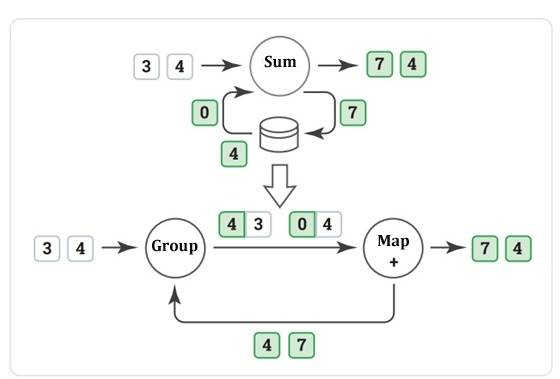
\includegraphics[width=.49\textwidth]{pics/classical-drifting}
  \caption{The comparison between typical state handling approach and drifting state model}
  \label {classical-drifting}
\end{figure}

\subsubsection{Properties}

In this setting, map operation is pure and order insensitive, and grouping operation is pure. Grouping operation is non-commutative because it should group a new element with the exact previous state. Hence, a straightforward approach to achieve determinism is to enforce order before each grouping in a data flow. Fortunately, grouping can be implemented optimistically. We assume that all elements arrive in-order. In this case, grouping handles out-of-order elements without blocking but possibly generating invalid output. A useful property of grouping operation is that generated invalid elements and descendants of these elements can be determined and their effects on the state of other groupings can be cleared. The scheme is shown in Figure~\ref{optimistic-grouping}. The numbers on this figure represent the right order of elements. An arriving element 3 is out-of-order. We know that invalid pair (1; 5) has been already released. In this case, the system generates valid pairs because the right position of the element 3 is determined. Besides, an invalid pair with a special flag is resent. Let us call such elements {\em sentinels}. While sentinels mostly behave as ordinary data items, their purpose is to seek and destroy previously released invalid pairs. Map operations handle sentinels as ordinary elements, but when a sentinel arrives at a grouping, it forces removing a corresponding invalid element from the bucket. Besides, actually valid pairs and new sentinels are sent further. Map functions are required to be pure in order to ensure that sentinels will go through exactly the same route as original pairs. An important property of invalid elements and corresponding sentinels is that they depend on the same input elements. This method is applicable to any number of subsequent groupings and guarantees that all groupings will eventually have a state as if all elements were in-order~\cite{we2018adbis}.
 
\begin{figure}[htbp]
  \centering
  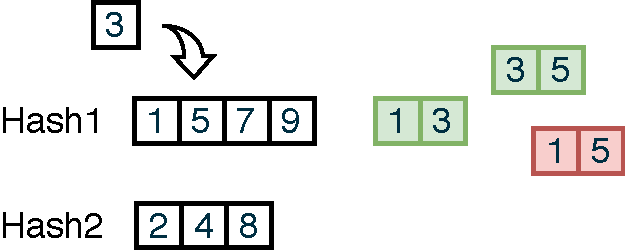
\includegraphics[width=.35\textwidth]{pics/grouping-invalidation}
  \caption{An idea of optimistic grouping implementation}
  \label {optimistic-grouping}
\end{figure} 

\subsection{Dependency tracking}

Invalid grouping items must be destroyed by sentinels to prevent inconsistent output. Hence, the system must hold invalid elements before releasing to end-user until all corresponding sentinels arrive. In drifting state model all output items are buffered in the very last node of the logical graph called {\em barrier}. The problem here is to detect that there are no in-flight sentinels for elements in the barrier and they will not be eventually generated. Invalid items and corresponding sentinels always depend on the same input element. Hence, if a system knows that all elements that depend on an input item are in the barrier, these elements can be delivered to end-user. 

Barriers require mechanisms for detecting dependencies between data flow elements. The well-known solution for dependency tracking is to inject special elements in a data flow. These elements go through the same path in a physical graph and "push through" preceding data flow elements. When such element arrives at the barrier, it means that buffered elements do not have in-flight dependencies. Flink checkpointing technique is based on this approach~\cite{Carbone:2017:SMA:3137765.3137777}. While it works well in systems that support only acyclic execution graphs, it is unclear how to handle such "pushing" elements in drifting state cycles. 

To solve this problem, each data item maintains a so-called {\em global time}: 

$$\forall{t\in{\mathbb{N}}, x\in{W_t}} : GT(x)=\Big[\frac{r(x)}{\Delta t}\Big].$$ 

Here, $\Delta t$ is the time quantum, that is possible to obtain on real hardware, e.g. 1 ms. The exact algorithms for computing and maintaining global time are detailed in~\cite{we2018adbis}, but the important property is that dependent in-flight elements have the same global time by the definition of $r(x)$. 

On each input item, an operation in a physical graph sends to the special agent called~{\em \Acker\ } global time together with checksum hashes of the input and output items. \Acker\ XORs all checksums grouped by global times and when the result becomes zero, it means that all items with a given global time were processed. In other words, it means that all descendants of an input element with the arrival time $GT$ are in the barrier. When such event occurs, \Acker\ broadcasts a notification to the subscribers, e.g. barriers. In this approach, collisions are possible, but they are very unlikely in practice. The idea of~\Acker\ is an adaptation of {\em Acker} from Apache Storm~\cite{apache:storm}.

Figure~\ref{acker} illustrates~\Acker\ functionality. Different shapes mean different data items. Green element is an input item. During processing, it is transformed into a blue item, and then the blue item is transformed into a yellow item. Yellow and blue items depend on the green item, so they all have the same global time (21). Each operation sends an ack for transformed items before ack for the input one to prevent XORed value become zero until all dependencies are in the barrier. For example, entry for global time 17 is zero, so it means that all dependencies of input element $a_{17}$ can be consistently released from the barrier, but for an input item $a_{21}$ there are still in-flight elements which depend on it.

\begin{figure}[htbp]
  \centering
  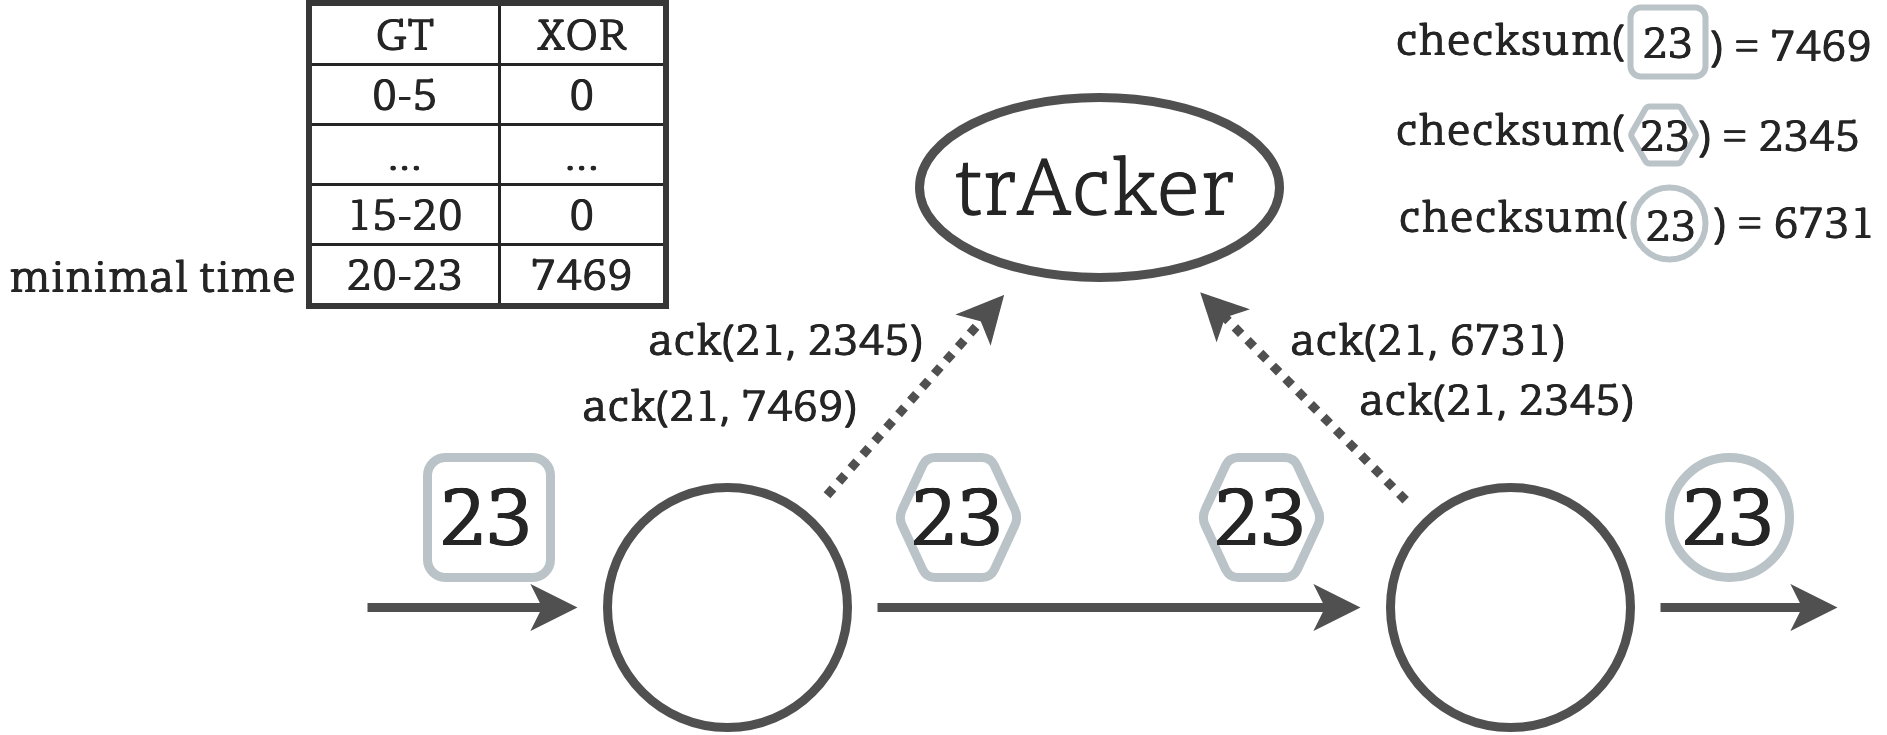
\includegraphics[scale=0.58]{pics/acker}
  \caption{The example of tracking dependencies using~\Acker\ }
  \label {acker}
\end{figure}

\subsection{Formal framework model}

According to the formal framework introduced above, the set of data flow elements in drifting state model consists of {\em data items}. Each data item contains user data called {\em payload} and global time that defines order.

$$DataItem=(Payload,GlobalTime)$$

Dependency relation $D$ is defined in the form of a possibly cyclic graph containing only map and grouping operations. The drifting state has the following important properties:

\begin{itemize}
    \item Total order enforcement and determinism with only a single buffer at the end of the data flow
    \item States of user operations are ordinary data items
    \item There is only a need to restore grouping buckets to recover processing 
\end{itemize}

Recovery mechanisms for drifting state model are detailed in the next section.
